\documentclass[a4paper,12pt]{article}

\usepackage{cmap}                   % поиск в PDF
\usepackage[T2A]{fontenc}           % кодировка
\usepackage[utf8]{inputenc}         % кодировка исходного текста
\usepackage[english,russian]{babel} % локализация и переносы
\usepackage[margin=1.5cm]{geometry}
%\usepackage{float}
\usepackage{graphicx} % картинки
\usepackage{wrapfig}
\usepackage{caption}
\usepackage{subcaption}
\usepackage{titling}

\author{Канушин Максим}
\title{Анализ разработанных задач в системе автоматической проверки для MOOC <<Программирование модулей ядра Linux>>}
\date{\today}

\begin{document} % Конец преамбулы, начало текста.

\setlength{\droptitle}{-75pt}
\maketitle
\section{Аннотация}
В данной работе исследуется статистика прохождения студентами массового открытого онлайн курса <<Программирование модулей ядра Linux>>\cite{stepic}. Проверка заданий, присланных студентами проходит в автоматическом режиме разработанной ранее системой. Задания представляют собой лабораторные работы, в рамках которых студенту необходимо разработать программу на языке С\cite{c} и Makefile\cite{makefile}. Целью исследования является определить насколько хорошо разработанные задачи и система их проверки соответствуют видео-лекциям и какие действия стоит предпринять, чтобы уменьшить количество студентов, бросающих онлайн-курс.

\section{Введение}
Многие студенты бросают онлайн-курсы когда перестают справляться с предложенными им заданиями или из-за того, что курс им надоедает и практические задания перестают быть им интересны. Для онлайн-курса <<Программирование модулей ядра Linux>> была разработана система, проверяющая корректность написанных студентами модулей ядра, которая позволила участникам курса загружать свои решения и в течение нескольких десятков секунд получать результаты проверки. Для того, чтобы улучшить онлайн-курс и уменьшить отток студентов, была проанализирована статистка тестового запуска курса. Целью исследования статистики являлось определить какие задачи тяжело даются студентам, а какие - наоборот легко и какие факторы могут на это влиять.


\section{Описание проверяющей системы}
Система автоматической проверки лабораторных работ представляет из себя комплекс взаимосвязанных программных средств, позволяющих студенту загрузить разработанную им программу и получить ответ о ее корректности, а так же логи сборки, запуска и информацию о произошедших ошибках при их наличии. Система обеспечивает изолированность проверяемого решения от внешней среды, чтобы обеспечить достаточный уровень надежности и безопасности исполнения. Помимо этого исключается взаимное влияние решений друг на друга для того, чтобы не дать возможность студенту случайно или намеренно повлиять на работу другого студента или просмотреть его. Среда, в которой происходит проверка, одинакова для всех решений, чтобы обеспечить как одинаковые условия проверки различных решений, так и многократную воспроизводимость результатов проверки одного и того же решения.

\section{Обзор результатов прохождения онлайн-курса}
Онлайн курс <<Программирование модулей ядра Linux>> был запущен в тестовом режиме. Курс состоял из 9 практических задач. В сумме по всем задачам было получено 795 решений из которых 270 правильных.

Статистика прохождения онлайн-курса представляла из себя csv-файл, содержащий информацию о всех загруженных решениях. Для ее обработки был создан набор скриптов на языке программирования Python\cite{python}. Для изучения статистики использовались следующие данные: идентификатор пользователя, идентификатор решаемой задачи, результат проверки и логи сборки, скрипта проверки и запуска решения. Скрипт позволил получить необходимые поля из csv-файла и посчитать метрики, описанные ниже.

\subsection{Stopout}

\begin{wrapfigure}[19]{L}{0.5\textwidth}
	\caption{Stopout}
	\centering
	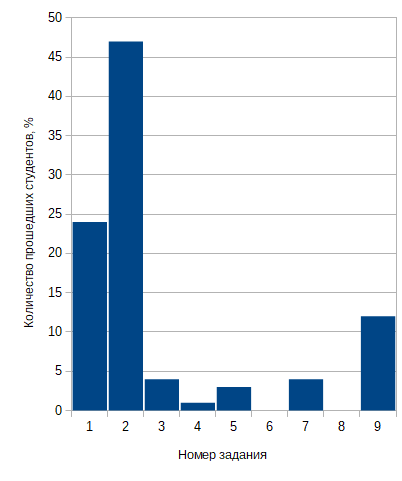
\includegraphics[width=0.4\textwidth]{stopout.png}
	\label{fig:mesh2}
\end{wrapfigure}

Stopout\cite{stopout}\cite{likelytostop} - величина, показывающая, сколько человек прекратили прохождение курса на той или иной задаче. Исследование этой характеристики позволит понять, какие задачи стоит усложнить, а какие, наоборот - сделать проще.

На рис. \ref{fig:mesh2} представлен график, показывающий распределение студентов, бросивших курс, по задачам до которых они добрались.

Первые два задания являются довольно простыми и схожими по сложности, что объясняет, почему многие студенты, выполнившие первое задание, решили и второе. Третье задание было заметно сложнее и большинство студентов бросили курс именно на ней. Данная метрика позволила понять, что разница в сложности между второй и третьей задачей слишком велика, что оттолкнуло студентов от продолжения курса.

\subsection{Пройденные студентами этапы в рамках задач}
По результатам проверки решений, были подсчитаны этапы в рамках каждой задачи, которые удалось пройти студенту. В общем случае выполнение любой задачи по курсу можно было разбить на 4 этапа: отправку файла с исходным кодом, сборку, загрузку собранного модуля в ядро и выполнение поставленных условий задачи. В ходе разработки скриптов и анализа статистики было обнаружено, что система в своем текущем виде не позволяет разбить задачу на большее число этапов, что позволило бы подробно исследовать проблемы каждой из задач.

Для каждого студента был посчитан шаг, на котором он бросил ту или иную задачу. На рис. \ref{fig:sub1} представлен график, показывающий какой процент студентов остановился на том или ином этапе задачи. Прохождение последнего этапа означает, что написанный модуль ядра полностью рабочий и выполняет все требования задания. Распределение по этому этапу выделено в отдельный график, представленный на рис. \ref{fig:sub2}. Данные, представленные для каждой задачи на обоих графиках, высчитывались относительно только тех студентов, которые приступили к ее выполнению.

Из графика на рис. \ref{fig:sub2} видно, что с каждой новой задачей, все больше студентов, которые брались за ее выполнение, старались довести ее до конца. Так же на графике \ref{fig:sub1} можно заметить, что с каждой новой задачей у студентов стали лучше получаться первые шаги, то есть все меньше студентов бросали решение задачи на неудавшейся сборке решения или загрузке модуля в ядро, и многие застревали именно на последнем, самом сложном  этапе, что означает, что разработанная система позволила многим студентам отработать общий навык написания модулей ядра и уменьшить количество совершаемых ими ошибок.

\begin{figure}
	\centering
	\begin{subfigure}{.5\textwidth}
		\centering
		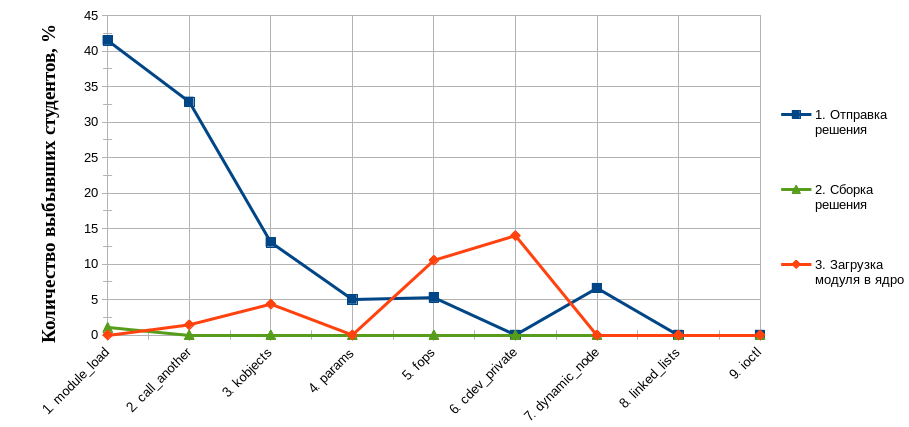
\includegraphics[width=\textwidth]{steps.png}
		\caption{}
		\label{fig:sub1}
	\end{subfigure}%
	\begin{subfigure}{.5\textwidth}
		\centering
		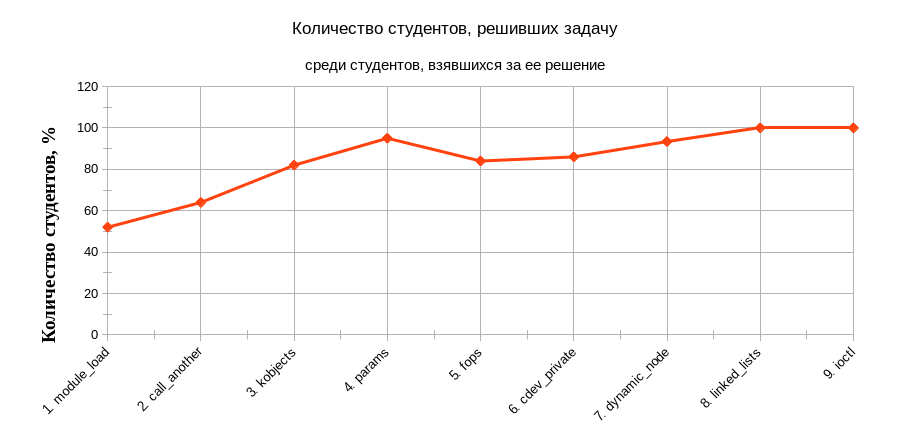
\includegraphics[width=\linewidth]{last_steps.png}
		\caption{}
		\label{fig:sub2}
	\end{subfigure}
	\caption{Распределение студентов по этапам, на которых они бросили задачу}
	\label{fig:mesh3}
\end{figure}

Поэтапное исследование решений задачи позволило понять, что в первых двух задачах курса, большинство студентов бросили задачу на самом первом этапе - неудавшейся сборке решения. Значительная разница в сложности между второй и третьей задачей курса оказалась не связана ни с одним из этапов их решения, так как большая часть студентов, взявшихся решать третью задачу, довели ее до конца. Данное наблюдение позволяет понять, что упрощение третьей задачи не даст должного эффекта и отток студентов не уменьшится. Вместо этого является целесообразным добавить дополнительную задачу, которая позволила бы студентам лучше усвоить тему и совершить более плавный переход к последующей задаче.

\section{Заключение}
В данной работе была изучена статистика тестового запуска онлайн-курса <<Программирование модулей ядра Linux>>. Анализ этой статистики показал, что большая часть студентов бросала курс дойдя до той или иной задачи, но не приступая к ее решению. Исследование этапов, на которых застряли студенты, позволило понять, что для улучшения задач курса необходимо доработать систему таким образом, чтобы для каждой задачи можно было выделить большее число этапов ее решения, чтобы понять где именно у студентов возникает больше всего проблем. Было решено, что после второй задачи целесообразно добавить еще одну - промежуточную, с целью уменьшения боязни студентов условий последующих задач и их оттока с курса.

\begin{thebibliography}{9}
	\bibitem{stepic} 
	Разработка модулей ядра Linux, // Stepik, URL:
	https://stepik.org/course/2051
	[Посещено: 15 Дек 2017]
	
	\bibitem{c}
	Kernighan, Brian W.; Ritchie, Dennis M.,
	The C Programming Language (1st ed.).,
	Englewood Cliffs 1978
	
	\bibitem{makefile}
	GNU Make,
	URL: https://www.gnu.org/software/make/
	[Посещено 17 Окт 2017]
	
	\bibitem{python}
	Python,
	URL: https://www.python.org/
	[Посещено: 8 Ноя 2017]
	
	\bibitem{likelytostop}
	{Taylor}, C. and {Veeramachaneni}, K. and {O'Reilly}, U.-M.
	\textit{Likely to stop? Predicting Stopout in Massive Open Online Courses}.
	ArXiv e-prints, 2014.
	
	\bibitem{stopout}
	Merriam-Webster dictionary,
	URL: https://www.merriam-webster.com/dictionary/
	[Посещено: 28 Ноя 2017]	
\end{thebibliography}

\end{document} % Конец текста.